\def\year{2022}\relax
%File: formatting-instructions-latex-2021.tex
%release 2021.2
\documentclass[letterpaper]{article} % DO NOT CHANGE THIS
\usepackage{aaai22}  % DO NOT CHANGE THIS
\usepackage{times}  % DO NOT CHANGE THIS
\usepackage{helvet} % DO NOT CHANGE THIS
\usepackage{courier}  % DO NOT CHANGE THIS
\usepackage[hyphens]{url}  % DO NOT CHANGE THIS
\usepackage{graphicx} % DO NOT CHANGE THIS
\urlstyle{rm} % DO NOT CHANGE THIS
\def\UrlFont{\rm}  % DO NOT CHANGE THIS
\usepackage{natbib}  % DO NOT CHANGE THIS AND DO NOT ADD ANY OPTIONS TO IT
\usepackage{caption} % DO NOT CHANGE THIS AND DO NOT ADD ANY OPTIONS TO IT
\usepackage{subcaption}
\frenchspacing  % DO NOT CHANGE THIS
\setlength{\pdfpagewidth}{8.5in}  % DO NOT CHANGE THIS
\setlength{\pdfpageheight}{11in}  % DO NOT CHANGE THIS
%\nocopyright

\usepackage{amsmath}
\usepackage{amsthm}
\usepackage{amssymb}
\newtheorem{theorem}{Theorem}
\newtheorem{corollary}{Corollary}
\newtheorem{lemma}{Lemma}
\newtheorem{observation}{Observation}
\newtheorem{definition}{Definition}
\newtheorem{example}{Example}

%PDF Info Is REQUIRED.
% For /Author, add all authors within the parentheses, separated by commas. No accents or commands.
% For /Title, add Title in Mixed Case. No accents or commands. Retain the parentheses.
% /Title ()
% Put your actual complete title (no codes, scripts, shortcuts, or LaTeX commands) within the parentheses in mixed case
% Leave the space between \Title and the beginning parenthesis alone
% /Author ()
% Put your actual complete list of authors (no codes, scripts, shortcuts, or LaTeX commands) within the parentheses in mixed case.
% Each author should be only by a comma. If the name contains accents, remove them. If there are any LaTeX commands,
% remove them.

% DISALLOWED PACKAGES
% \usepackage{authblk} -- This package is specifically forbidden
% \usepackage{balance} -- This package is specifically forbidden
% \usepackage{color (if used in text)
% \usepackage{CJK} -- This package is specifically forbidden
% \usepackage{float} -- This package is specifically forbidden
% \usepackage{flushend} -- This package is specifically forbidden
% \usepackage{fontenc} -- This package is specifically forbidden
% \usepackage{fullpage} -- This package is specifically forbidden
% \usepackage{geometry} -- This package is specifically forbidden
% \usepackage{grffile} -- This package is specifically forbidden
% \usepackage{hyperref} -- This package is specifically forbidden
% \usepackage{navigator} -- This package is specifically forbidden
% (or any other package that embeds links such as navigator or hyperref)
% \indentfirst} -- This package is specifically forbidden
% \layout} -- This package is specifically forbidden
% \multicol} -- This package is specifically forbidden
% \nameref} -- This package is specifically forbidden
% \usepackage{savetrees} -- This package is specifically forbidden
% \usepackage{setspace} -- This package is specifically forbidden
% \usepackage{stfloats} -- This package is specifically forbidden
% \usepackage{tabu} -- This package is specifically forbidden
% \usepackage{titlesec} -- This package is specifically forbidden
% \usepackage{tocbibind} -- This package is specifically forbidden
% \usepackage{ulem} -- This package is specifically forbidden
% \usepackage{wrapfig} -- This package is specifically forbidden
% DISALLOWED COMMANDS
% \nocopyright -- Your paper will not be published if you use this command
% \addtolength -- This command may not be used
% \balance -- This command may not be used
% \baselinestretch -- Your paper will not be published if you use this command
% \clearpage -- No page breaks of any kind may be used for the final version of your paper
% \columnsep -- This command may not be used
% \newpage -- No page breaks of any kind may be used for the final version of your paper
% \pagebreak -- No page breaks of any kind may be used for the final version of your paperr
% \pagestyle -- This command may not be used
% \tiny -- This is not an acceptable font size.
% \vspace{- -- No negative value may be used in proximity of a caption, figure, table, section, subsection, subsubsection, or reference
% \vskip{- -- No negative value may be used to alter spacing above or below a caption, figure, table, section, subsection, subsubsection, or reference

\setcounter{secnumdepth}{0} %May be changed to 1 or 2 if section numbers are desired.

% The file aaai21.sty is the style file for AAAI Press
% proceedings, working notes, and technical reports.
%

% Title

% Your title must be in mixed case, not sentence case.
% That means all verbs (including short verbs like be, is, using,and go),
% nouns, adverbs, adjectives should be capitalized, including both words in hyphenated terms, while
% articles, conjunctions, and prepositions are lower case unless they
% directly follow a colon or long dash


%Example, Single Author, ->> remove \iffalse,\fi and place them surrounding AAAI title to use it
\title{Social Aware Assignment of Passengers in Ridesharing}
\author {
    % Authors
    Chaya Levinger, %\textsuperscript{\rm 1}
    Noam Hazon, % \textsuperscript{\rm 2}
    Amos Azaria% \textsuperscript{\rm 3} \\
}
\affiliations {
    % Affiliations
    %\textsuperscript{\rm 1,2,3}
    Department of Computer Science, Ariel University, Ariel, Israel 4070000 \\
    chaya.levinger@msmail.ariel.ac.il,
    noamh@ariel.ac.il,
    amos.azaria@ariel.ac.il
}


% \iffalse
% %Example, Multiple Authors, ->> remove \iffalse,\fi and place them surrounding AAAI title to use it
% \title{My Publication Title --- Multiple Authors}
% \author {
%     % Authors
%     First Author Name,\textsuperscript{\rm 1}
%     Second Author Name, \textsuperscript{\rm 2}
%     Third Author Name \textsuperscript{\rm 1} \\
% }
% \affiliations {
%     % Affiliations
%     \textsuperscript{\rm 1} Affiliation 1 \\
%     \textsuperscript{\rm 2} Affiliation 2 \\
%     firstAuthor@affiliation1.com, secondAuthor@affilation2.com, thirdAuthor@affiliation1.com
% }
% \fi





\usepackage[ruled,noend,linesnumbered]{algorithm2e}
%\usepackage{hhline}
%\usepackage{enumitem}
\usepackage{amsthm}
%\usepackage{diagbox}
%\usepackage{url}
%\usepackage{graphicx}
\usepackage{breqn}
\usepackage{tikz}
\usetikzlibrary{arrows,positioning,automata}
\usepackage{braket}






\begin{document}

\maketitle

\begin{abstract}
    We analyze the assignment of passengers in a shared ride, which considers the social relationship among the passengers. Namely, there is a fixed number of passengers in each vehicle, and the goal is to recommend an assignment of the passengers such that the number of friendship relations is maximized. We show that the  problem is computationally hard, and we provide an approximation algorithm.
\end{abstract}

%%
%% The code below is generated by the tool at http://dl.acm.org/ccs.cfm.
%% Please copy and paste the code instead of the example below.
%%

\section{Introduction}
%start with the example


Coalition formation is an important research branch within multiagent systems~\cite{chalkiadakis2011computational}.
It analyses the outcome that results when a set of agents is partitioned into coalitions.
For example, consider a group of travelers (passengers) who want to reach a similar destination. Each passenger has a preference related to who will be with her in the vehicle. Namely, each passenger would rather share a vehicle with as many of her friends during the ride, and thus the utility of each passenger is the number of friends traveling with her.  However, the vehicles have a limited capacity. The goal is to assign the passengers to vehicles while maximizing the social welfare (the sum of all passengers' utilities).
%another example is: dormitories / office rooms. tasks

We formulate the described problem as the social aware assignment problem, which assumes that the agents' utilities depend on a social network that represents the social relationships among the agents. The
social network is modeled as an unweighted graph where the
vertices are agents and the edges indicate friendship among
the agents. The utility function of an agent is the number
of friends she has within the coalition to which she is assigned.
In addition, there is a hard constraint on the maximal size of each coalition.
Actually, our model is a special case of simple Additively
Separable Hedonic Games (ASHGs) \cite{bogomolnaia2002stability}.
In this paper, we show that the social aware assignment problem is computationally hard, and we provide an approximation algorithm.

\section{Related Work}
Sless et al. \shortcite{sless2018forming} tackle a problem similar to ours. Similar to our work, they assume a friendship graph and attempt to maximize the number of friends in each group. However, in their setting the agents must be partitioned into exactly $k$ groups without any restriction on each group's size. The graph partitioning problem, introduced by Hyafil and Rivest~\shortcite{hyafil1973graph}, is a more restricted problem, in which the vertices of a graph must be partitioned into exactly $k$ groups of equal sizes. % such that few edges cross between sets. %They show that the problem is NP-complete.
%\cite{hendrickson1995multi}.

Wright and Vorobeychik \shortcite{wright2015mechanism} also study a model of ASHG where there is a restriction on the size of each coalition. Within their model, they propose a strategyproof mechanism that achieves good and fair experimental performance, despite not having a theoretical guarantee.

\section{The Social Aware Assignment Problem}
We analyze the problem of the assignment in ride-sharing problem, while maintaining the human-centric approach.
Specifically, our goal is to assign the users to vehicles such that each user will be matched with as many friends as possible in the same vehicle, while each vehicle is limited to a number of passengers, $k$. Formally,


\begin{definition}[Social aware assignment]
We are given a number $k$ and an undirected friendship graph $G=(U,E)$ where $(u_i, u_j) \in E$ if the user $u_i$ and the user $u_j$ are friends of each other. The goal is to find an assignment $P$, which is a partition of the set $U$, such that $\forall S\in P, |S|\leq k$, and the value of $P$, $V_P = |\{(u_i, u_j) \in E \mbox{: } \exists S \in P \mbox{ where } u_i \in S \mbox{ and } u_j \in S\}|$ is maximized.
\end{definition}
For example, given the graph in Figure \ref{fig:Graph} and a vehicle size limit $k=3$, the value of the partition $P = \{\{v_1,v_3,v_6\}, \allowbreak \{v_2,v_4,v_7\}, \{v_5,v_8\}\}$, shown in Figure~\ref{fig:Partition}, equals $7$. Indeed, this is the optimal partition since there is no other partition with higher value.
Clearly, the decision variant of the social aware assignment problem is to decide whether there exists a partition with a value of at least $\upsilon$.


%The answer of the decision variant of the social aware assignment problem is $true$ for each $\kappa \leq 7$ and $false$ otherwise.\\


\begin{figure}
     \centering
     \begin{subfigure}{0.45\textwidth}
         \centering
         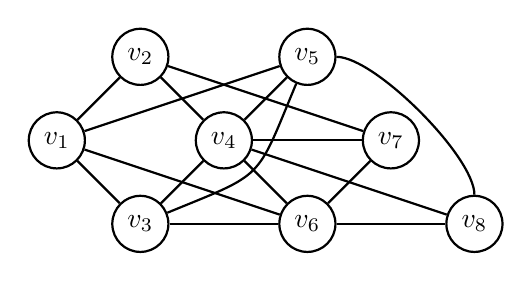
\begin{tikzpicture}[node distance={15mm}, thick, main/.style = {draw, circle}] {Graph}
            \node[main] (a) {$v_1$};
            \node[main] (b) [above right of=a] {$v_2$};
            \node[main] (c) [below right of=a] {$v_3$};
            \node[main] (d) [above right of=c] {$v_4$};
            \node[main] (e) [above right of=d] {$v_5$};
            \node[main] (f) [below right of=d] {$v_6$};
            \node[main] (g) [below right of=e] {$v_7$};
            \node[main] (h) [below right of=g] {$v_8$};
            \draw (a) -- (b);
            \draw (a) -- (c);
            \draw (a) -- (e);
            \draw (b) -- (d);
            \draw (c) -- (d);
            \draw (e) -- (d);
            \draw (e) to [out=247.5, in=22.5, looseness=1.5] (c);
            \draw (f) -- (d);
            \draw (g) -- (f);
            \draw (g) -- (d);
            \draw (f) -- (a);
            \draw (g) -- (b);
            \draw (e) to [out=360, in=90, looseness=0.5] (h);
            \draw (h) -- (d);
            \draw (h) -- (f);
            \draw (c) -- (f);
        \end{tikzpicture}
        \caption{The graph $G$}
        \label{fig:Graph}
     \end{subfigure}
     \hfill
     \begin{subfigure}{0.45\textwidth}
         \centering
         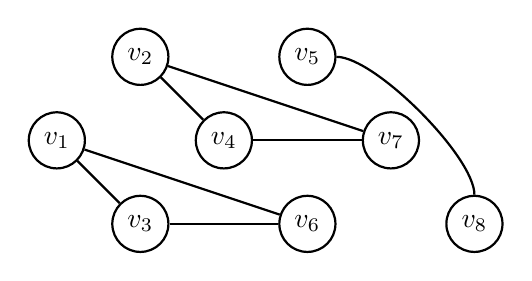
\begin{tikzpicture}[node distance={15mm}, thick, main/.style = {draw, circle}] {Graph}
            \node[main] (a) {$v_1$};
            \node[main] (b) [above right of=a] {$v_2$};
            \node[main] (c) [below right of=a] {$v_3$};
            \node[main] (d) [above right of=c] {$v_4$};
            \node[main] (e) [above right of=d] {$v_5$};
            \node[main] (f) [below right of=d] {$v_6$};
            \node[main] (g) [below right of=e] {$v_7$};
            \node[main] (h) [below right of=g] {$v_8$};
            \draw (a) -- (c);
            \draw (f) -- (a);
            \draw (c) -- (f);
            \draw (b) -- (d);
            \draw (g) -- (d);
            \draw (g) -- (b);
            \draw (e) to [out=360, in=90, looseness=0.5] (h);
        \end{tikzpicture}
        \caption{An optimal partition of $G$}
        \label{fig:Partition}
    \end{subfigure}
    \caption{An example for the social aware assignment problem where $k=3$.}
    \label{}
\end{figure}

\section{The Hardness of the Social Aware Assignment Problem}
The social aware assignment problem when $k=2$ is equivalent to the maximum matching problem, and thus it can be computed in polynomial time \cite{edmons1965paths}.
However, our problem becomes intractable when $k \geq 3$.
%For the hardness proof we use the problem of partition into triangles, which was shown to be in $NP$-Complete \cite{di2004np}.
% Specifically, in this problem the goal is to decide whether the vertices of a graph $G$ can be partitioned into $q$ disjoint sets $V_1, V_2, . . . , V_q$, each containing exactly $3$ vertices, such that each of these $V_i$ is the node set of a triangle in $G$.
For the hardness proof, we define for each $k \in \mathbb{N}$ the $Cliques_k$ problem, which is as follows.
\begin{definition}[$Cliques_k$]
Given an undirected graph $G=(V,E)$, decide whether $V$ can be partitioned into disjoint cliques, such that each clique is composed of exactly $k$ vertices.
\end{definition}
Clearly, $Cliques_2$ can be decided in polynomial time by computing a maximum matching of the graph $G$, $M$, and testing whether $|M| = \frac{|V|}{2}$.
However, $Cliques_k$ becomes hard when $k\geq 3$.
\begin{lemma}
$Cliques_k$ is in $NP$-Complete for every $k\geq3$.
\end{lemma}
% \begin{proof}
% Clearly, $Cliques_k$ is in $NP$ for every $k$.
% We use induction to show that any $Cliques_k$ is in $NP$-Hard for every $k\geq 3$.
% $Cliques_3$ is known as the `partition into triangles' problem, which was shown to be in $NP$-Complete \cite{di2004np}.
% Given that $Cliques_k$ is in $NP$-Hard we show that $Cliques_{k+1}$ is also in $NP$-Hard.
% Given an instance of the $Cliques_k$ on a graph $G(V,E)$, we construct the following instance. We build a graph $G'(V',E')$, in which we add a set of nodes $\hat{V} = {\hat{v}_1, ..., \hat{v}_{\frac{|V|}{k}}}$, i.e., $V' = V \cup \hat{V}$. If $e \in E$ then $e \in E'$, and for every $v \in V, \hat{v} \in \hat{V}$ we add $(v,\hat{v})$ to $E'$.
% %Clearly, $Cliques_\kappa(G) = Cliques_{\kappa+1}(G')$.
% Clearly, $V$ can be partitioned into disjoint cliques with exactly $k$ vertices if and only if $V'$ can be partitioned into disjoint cliques with  exactly $k+1$ vertices.
% \end{proof}


\begin{theorem}
The decision variant of the social aware assignment problem is in $NP$-Complete.
\end{theorem}
%\begin{proof}
%Clearly the problem is in $NP$, since if we are given a partition $P$, a limit $k$ and the value $\upsilon$, we can easily check that $\forall  U \in P$, $|U| \leq k$ and the value of $P$, $V_P \geq \upsilon$ in polynomial time. For the hardness proof we use the $Cliques_k$ problem.
%Given an instance of $Cliques_k$ on a graph $G(V,E)$, we use the same graph with the same $k$ and $\upsilon = \frac{|V|(k-1)}{2}$ as an instance to the social aware assignment problem. Clearly, $V$ can be partitioned into disjoint cliques with exactly $k$ vertices if and only if there exist a partition $P$ such that $\forall S\in P, |S|\leq k$, and $V_P = \upsilon$.
%\end{proof}

\section{Approximation of the Social Aware Assignment Problem}
Since we showed that the social aware assignment problem is in $NP$-Complete, we first provide an approximation algorithm where $k=3$.
The algorithm works as follows. It first computes a maximum matching, $M$, in the given graph $G$. It then creates a graph $G'$ that includes all the unmatched nodes and a union node for each pair of matched nodes in $M$. Finally, it computes a maximum matching in $G'$ and returns the partition, $P$, of all the matched sets.
% For example, given the graph $G$ in Figure \ref{fig:G}, the algorithm finds some maximum matching, e.g the matching $M = \{(v_1,v_2),(v_3,v_4)\}$ shown in Figure \ref{fig:M}.  It then creates the graph $G'$ in Figure \ref{fig:G'} and finds some maximum match in it. For the matching $M'=\{(v_{3,4}, v_5)\}$ it returns the partition $P={\{v_1,v_2\},\{v_3,v_4,v_5\},\{v_6\}}$ shown in Figure \ref{fig:P}.

 % \begin{enumerate}
    %     \item Given a graph $G=(V,E)$, find a maximum matching, $M$, in $G$. %\cite{duan2014linear}.
    %     \item Create an undirected graph $G' = (V',E')$ such that $\forall (v_i, v_j) \in M$. Create a node $v_{i,j} \in V'$ and $\forall v_i \in V$, $v_i \in V'$ if there is no $v_j \in V$ such that $(v_i,v_j) \in M$.
    %     In addition, $\forall v_{i,j}, v_k \in V'$, $(v_{i,j}, v_k) \in E'$ if $(v_i,v_k) \in E$ or $(v_j,v_k) \in E$ %$\forall v_i,v_j \in V', (v_i,_j) \in E'$ if $ (v_i,v_j) \in E$ and
    %     \item Find a maximum matching in $G'$.
    % \end{enumerate}



    \begin{algorithm}[ht]
        \caption{Approximation algorithm for $k$=3}
        \label{alg:approximation}
        \SetAlgoLined
        \textbf{Input}:
        A graph $G=(V,E)$\\
        \KwResult{A partition $P$ of $G$ where $k=3$.}
        M $\leftarrow$ maximum matching in $G$\\
        $G'=(V',E') \leftarrow$ an empty graph\\
        \For{\upshape every $(v_i, v_j) \in M$}{
            Add vertex $v_{i,j}$ to $G'$\\
            remove $v_i, v_j$ from $V$
        }
        \For{\upshape every $v_i \in V$}{
                Add vertex $v_i$ to $G'$
        }
        \For{\upshape every $(v_i, v_j) \in M$}{
            \For{\upshape every $v_k \in V$}{
                \If {\upshape $(v_i, v_k) \in E$ OR $(v_j, v_k) \in E$}{
                    Add edge $(v_{i,j}, v_k)$ to $G'$
                }
            }
        }
        $M' \leftarrow$ maximum matching in $G'$\\
        $P \leftarrow$ an empty partition\\
        \For{\upshape every $(v_{i,j}, v_k) \in M'$}{
            add the set $\{v_i, v_j, v_k\}$ to P\\
            remove $(v_i,v_j)$ from $M$\\
            remove $v_k$ from $V$\\
        }
        \For{\upshape every $(v_i,v_j) \in M$}{
            add the set $\{v_i, v_j\}$ to P
        }
        \For{\upshape every $v_i \in V$}{
            add the set $\{v_i\}$ to P
        }
        \textbf{return} P
    \end{algorithm}

    % \begin{figure}[ht]
    %     \centering
    %     \begin{minipage}{.45\textwidth}
    %         \centering
    %         \begin{tikzpicture}[node distance={12mm}, thick, main/.style = {draw, circle}] {Graph}
    %         \node[main] (1) {$v_1$};
    %         \node[main] (2) [above right of=1] {$v_2$};
    %         \node[main] (3) [below right of=1] {$v_3$};
    %         \node[main] (4) [above right of=3] {$v_4$};
    %         \node[main] (5) [above right of=4] {$v_5$};
    %         \node[main] (6) [below right of=4] {$v_6$};
    %         \draw (1) -- (2);
    %         \draw (3) -- (2);
    %         \draw (3) -- (4);
    %         \draw (4) -- (5);
    %         \draw (4) -- (6);
    %         \end{tikzpicture}
    %         \caption{The graph G}
    %         \label{fig:G}
    %     \end{minipage}
    %     \begin{minipage}{.45\textwidth}
    %         \centering
    %         \begin{tikzpicture}[node distance={12mm}, thick, main/.style = {draw, circle}] {Graph}
    %         \node[main] (1) {$v_1$};
    %         \node[main] (2) [above right of=1] {$v_2$};
    %         \node[main] (3) [below right of=1] {$v_3$};
    %         \node[main] (4) [above right of=3] {$v_4$};
    %         \node[main] (5) [above right of=4] {$v_5$};
    %         \node[main] (6) [below right of=4] {$v_6$};
    %         \draw (1) -- (2);
    %         \draw (3) -- (4);
    %         \end{tikzpicture}
    %         \caption{The Matching M}
    %         \label{fig:M}
    %     \end{minipage}
    %     \begin{minipage}{.45\textwidth}
    %         \centering
    %         \begin{tikzpicture}[node distance={12mm}, thick, main/.style = {draw, circle}] {Graph}
    %         \node[main] (12) {$v_{1,2}$};
    %         \node[main] (34) [below right of=12] {$v_{3,4}$};
    %         \node[main] (5) [above right of=34] {$v_5$};
    %         \node[main] (6) [below right of=34] {$v_6$};
    %         \draw (34) -- (5);
    %         \draw (34) -- (6);
    %         \end{tikzpicture}
    %         \caption{The graph G'}
    %         \label{fig:G'}
    %     \end{minipage}
    %     \begin{minipage}{.45\textwidth}
    %         \centering
    %         \begin{tikzpicture}[node distance={12mm}, thick, main/.style = {draw, circle}] {Graph}
    %         \node[main] (1) {$v_1$};
    %         \node[main] (2) [above right of=1] {$v_2$};
    %         \node[main] (3) [below right of=1] {$v_3$};
    %         \node[main] (4) [above right of=3] {$v_4$};
    %         \node[main] (5) [above right of=4] {$v_5$};
    %         \node[main] (6) [below right of=4] {$v_6$};
    %         \draw (1) -- (2);
    %         \draw (3) -- (4);
    %         \draw (4) -- (5);
    %         \end{tikzpicture}
    %         \caption{The partition P}
    %         \label{fig:P}
    %     \end{minipage}
    % \end{figure}

%We first present a theoretical procedure that, given an optimal partition $Opt$ and $G'$, finds a matching with a size of at least $\frac{|V|-2|M|-|O|}{2}$. Where $O=\{v_o$ s.t. $\{v_o\} \in Opt\}$. We will show that Algorithm \ref{alg:approximation} is guaranteed to perform at least as well as this procedure, which results in an approximation ratio of $0.5$ for $k=3$.
%Without loss of generality, we assume that every set $S \in Opt$ is a connected component.

% \begin{algorithm}[ht]
%     \caption{Find_matching}
%     \label{alg:findMatch}
%     \SetAlgoLined
%     \textbf{Input}:\\
%     The optimal partition $Opt$\\
%     %A partition into triangles $T$\\
%     A graph $G'=(V',E')$\\
%     \KwResult{A matching in $G'$}
%     $R \leftarrow$ an empty matching\\
%     \For {\upshape each $v_i$ such that $\{v_i\} \in Opt$}
%         {remove $v_i$ from $V'$}
%     \For{\upshape each $v_i \in V'$}{
%         let $\hat{v}$ be $v_{j,k}$ or $v_{k,j}$ such that $v_i$ and $v_j$ belong to the same set in $Opt$ and $(v_i, \hat{v})\in E'$\\
%             %\If{\upshape $\{v_i, v_j, v_k\} \notin Opt$}{
%                 \For {\upshape each $v_l \neq v_i$ such that $v_j, v_l$ belong to the same set in $Opt$}{
%                     remove $v_l$ from $V'$ }
%                 \For {\upshape each $v_l \neq v_i$ such that $v_k, v_l$ belong to the same set in $Opt$ and $(v_l,\hat{v})\in E'$}{
%                 remove $v_l$ from $V'$ }
%             %}
%         add $(v_i, \hat{v})$ to $R$
%     }
%     \textbf{return} $R$
% \end{algorithm}

%We want to show that even in this situation, when $k=3$, Then, algorithm \ref{alg:approximation} provides a solution for the social aware assignment problem with an approximation ratio of $0.5$.


\begin{theorem}
For $k=3$, Algorithm \ref{alg:approximation} provides a solution for the social aware assignment problem with an approximation ratio of $0.5$.
\end{theorem}

% \begin{proof}
% The size of the optimal solution is at most the size of the partition into triangles of all the node except the group $O$, that is, $|V|-|O|$.
% Clearly, $|P| \geq |M| + |M'|$.
% By definition, $M'$ is a maximum matching in $G'$ and thus $|M'| \geq |R|$.
% Therefore, $|P| \geq |M| + |R| \geq |M| + \frac{|V|-2|M|-|O|}{2} = \frac{|V|-|O|}{2} \geq \frac{|Opt|}{2}$.
% \end{proof}


%  \begin{figure}
%      \centering
%     \begin{tikzpicture}[>=stealth',shorten >=1pt,node distance=3cm,on grid,initial/.style    ={}]
%         \node[draw,circle] (j) at (0, 0.5)  {$v_j$};
%         \node[draw,circle] (k) at (0, -0.5)  {$v_k$};
%         \node[draw,circle] (i) at (-1,1.5)  {$v_i$};
%         \node[draw,circle] (l) at (-3.5, 0)  {$v_l$};
%         \draw (0,0) ellipse (0.8cm and 1cm);
%         \node at (0.5,0) {$\hat{v}$};
%         \draw (i) -- (j);
%         \draw (j) -- (k);
%         \tikzset{mystyle/.style={color=black}}
%         \tikzset{every node/.style={fill=white}}
%         \path (l)     edge [mystyle]    node   {$line 10$} (j)
%               (l)     edge [mystyle]    node   {$line 12$} (k);
%     \end{tikzpicture}
%     \caption{}
%     \label{}
%  \end{figure}

% Next, we provide a procedure that attempts to model the behavior of the passengers in the social aware assignment problem when there is no central mechanism that determines the assignment and $k=3$. Assume that the users are split up arbitrarily but maximally, i.e., in a way that there are no additional connections that can be added. We call this procedure $Arbmax$.
% Without loss of generality, we assume that every set $S \in Arbmax$ is a connected component.
% %We show that the uncoordinated procedure may result in an approximation ratio of only $\frac{1}{3}$; however, we show that a ratio of $\frac{1}{3}$ is guaranteed.
% We show that the worst case scenario of $Arbmax$ provides an approximation of $\frac{1}{3}$.
% %
% % Figure \ref{fig:1/3 scenario} presents a case where $Arbmax$ provides an approximation of exactly $\frac{1}{3}$. Where $Arbmax = \{\{v_1, v_4, v_7\}, \{v_2\}, \{v_3\}, \{v_5\}, \{v_6\}, \{v_8\}, \{v_9\}\}$ and $|Arbmax| = 2$ and $Opt = \{\{v_1, v_2, v_3\}, \{v_4, v_5, v_6\}, \{v_7, v_8, v_9\}\}$ and $|Opt| = 6$.
% %
% %
% %  \begin{figure}[ht]
% %      \centering
% %     \begin{tikzpicture}[node distance={12mm}, thick, main/.style = {draw, circle}] {Graph}
% %     \node[main] (1) {$v_1$};
% %     \node[main] (2) [above  left of=1] {$v_2$};
% %     \node[main] (3) [above right of=1] {$v_3$};
% %     \node[main] (7) [below right of=3] {$v_7$};
% %     \node[main] (8) [below left of=7] {$v_8$};
% %     \node[main] (9) [below right of=7] {$v_9$};
% %     \node[main] (5) [above right of=7] {$v_5$};
% %     \node[main] (4) [below right of=5] {$v_4$};
% %     \node[main] (6) [above right of=4] {$v_6$};
% %     \draw (1) -- (2);
% %     \draw (1) -- (3);
% %     \draw (5) -- (4);
% %     \draw (4) -- (6);
% %     \draw (7) -- (8);
% %     \draw (7) -- (9);
% %     \draw (1) -- (7);
% %     \draw (4) -- (7);
% %     \end{tikzpicture}
% %     \caption{}
% %     \label{fig:1/3 scenario}
% %  \end{figure}
% %
% Indeed, $Arbmax$ is guaranteed to provide an approximation  ratio of $\frac{1}{3}$.
% \begin{theorem}
% $Arbmax$ provides an approximation with a ratio of $\frac{1}{3}$, and this ratio is tight.
% \end{theorem}


%\subsection{Approximation of the Social Aware Assignment Problem for General k}
Similarly to the approximation algorithm where $k=3$, we provide the Match and Merge (MnM) algorithm, which is an approximation algorithm for any $k \geq 3$.
The algorithm consists of $k-1$ rounds. Each round is composed of a matching phase followed by a merging phase.
Specifically, in round $l$ MnM computes a maximum matching, $M_l \subseteq E_l$, for $G_l$ (where $G_1 = G$). In the merging phase, MnM creates a graph $G_{l+1}$ that includes a merged node for each pair of matched nodes. $G_{l+1}$ also includes all unmatched nodes, along with their edges to the merged nodes.
Finally, MnM returns the partition, $P$, of all the matched sets.
\begin{theorem}
For $k>3$, MnM provides an approximation ratio of $\frac{1}{k-1}$ for the social aware assignment problem.
\end{theorem}
% For example, given the graph $G_1$ in Figure \ref{fig:G_1} and $k=4$, the algorithm finds some maximum matching, e.g the matching $M_1 = \{(v_1,v_2),(v_3,v_4)\}$ shown in Figure \ref{fig:M}.  It then creates the graph $G_2$ in Figure \ref{fig:G_2} and finds some maximum match in it. e.g the matching $M_2 = \{(v_{3,4},v_5)\}$ shown in Figure \ref{fig:M_2}. It then creates the graph $G_3$ in Figure \ref{fig:G_3} and finds some maximum match in it. For the matching $M_3=\{(v_{3,4,5}, v_6)\}$ it returns the partition $P={\{v_1,v_2\},\{v_3,v_4,v_5,v_6\}}$ shown in Figure \ref{fig:PforK=4}.

% \begin{algorithm}[ht]
%     \caption{Approximation for $k\geq3$}
%     \label{alg:approximationFork>3}
%     \SetAlgoLined
%     \textbf{Input}:
%     A graph $G_1=(V_1,E_1)$\\
%     \KwResult{A partition $P$ of $G_1$.}
%     \For{$l\leftarrow1$ to $k-1$}{
%         $M_l$ $\leftarrow$ maximum matching in $G_l$\\
%         $G_{l+1}=(V_{l+1},E_{l+1}) \leftarrow$ an empty graph\\
%         $V_{l+1} \leftarrow V_l$\\
%         \For{\upshape every $(v_{i_1,...,i_l}, v_j) \in M_l$}{
%             Add vertex $v_{i_1,...,i_l,j}$ to $V_{l+1}$\\
%             remove $v_{i_1,...,i_l}, v_j$ from $V_{l+1}$
%         }
%         \For{\upshape every $(v_{i_1,...,i_l}, v_j) \in M_l$}{
%             \For{\upshape every $v_m \in V_{l+1}$}{
%                 \If {\upshape $(v_{i_1,...,i_l}, v_m) \in E_l$ OR $(v_j, v_m) \in E_l$}{
%                     Add $(v_{i_1,...,i_l,j}, v_m)$ to $E_{l+1}$
%                 }
%             }
%         }
%     }
%     $P \leftarrow$ an empty partition\\
%     \For{\upshape every $v_i \in V_1$}{
%         add the set $\{v_i\}$ to $P$
%     }
%     \For{$l \leftarrow 1$ to $k-1$}{
%         \For{\upshape every $(v_{i_1,...,i_{l}}, v_j) \in M_l$}{
%             add the set $\{v_{i_1},...,v_{i_l},v_j\}$ to $P$\\
%             remove $\{v_{i_1,...,i_{l}}\}, \{v_j\}$ from $P$\\
%         }
%     }
%     \textbf{return} P
% \end{algorithm}

    % \begin{figure}[ht]
    %     \centering
    %     \begin{minipage}{.45\textwidth}
    %         \centering
    %         \begin{tikzpicture}[node distance={12mm}, thick, main/.style = {draw, circle}] {Graph}
    %         \node[main] (1) {$v_1$};
    %         \node[main] (2) [above right of=1] {$v_2$};
    %         \node[main] (3) [below right of=1] {$v_3$};
    %         \node[main] (4) [above right of=3] {$v_4$};
    %         \node[main] (5) [above right of=4] {$v_5$};
    %         \node[main] (6) [below right of=4] {$v_6$};
    %         \draw (1) -- (2);
    %         \draw (3) -- (2);
    %         \draw (3) -- (4);
    %         \draw (4) -- (5);
    %         \draw (4) -- (6);
    %         \end{tikzpicture}
    %         \caption{The graph $G_1$}
    %         \label{fig:G_1}
    %     \end{minipage}
    %     \begin{minipage}{.45\textwidth}
    %         \centering
    %         \begin{tikzpicture}[node distance={12mm}, thick, main/.style = {draw, circle}] {Graph}
    %         \node[main] (1) {$v_1$};
    %         \node[main] (2) [above right of=1] {$v_2$};
    %         \node[main] (3) [below right of=1] {$v_3$};
    %         \node[main] (4) [above right of=3] {$v_4$};
    %         \node[main] (5) [above right of=4] {$v_5$};
    %         \node[main] (6) [below right of=4] {$v_6$};
    %         \draw (1) -- (2);
    %         \draw (3) -- (4);
    %         \end{tikzpicture}
    %         \caption{The Matching $M_1$}
    %         \label{fig:M_1}
    %     \end{minipage}
    %     \begin{minipage}{.45\textwidth}
    %         \centering
    %         \begin{tikzpicture}[node distance={12mm}, thick, main/.style = {draw, circle}] {Graph}
    %         \node[main] (12) {$v_{1,2}$};
    %         \node[main] (34) [below right of=12] {$v_{3,4}$};
    %         \node[main] (5) [above right of=34] {$v_5$};
    %         \node[main] (6) [below right of=34] {$v_6$};
    %         \draw (34) -- (5);
    %         \draw (34) -- (6);
    %         \end{tikzpicture}
    %         \caption{The graph $G_2$}
    %         \label{fig:G_2}
    %     \end{minipage}
    %     \begin{minipage}{.45\textwidth}
    %         \centering
    %         \begin{tikzpicture}[node distance={12mm}, thick, main/.style = {draw, circle}] {Graph}
    %         \node[main] (12) {$v_{1,2}$};
    %         \node[main] (34) [below right of=12] {$v_{3,4}$};
    %         \node[main] (5) [above right of=34] {$v_5$};
    %         \node[main] (6) [below right of=34] {$v_6$};
    %         \draw (34) -- (5);
    %         \end{tikzpicture}
    %         \caption{The Matching $M_2$}
    %         \label{fig:M_2}
    %     \end{minipage}
    %     \begin{minipage}{.45\textwidth}
    %         \centering
    %         \begin{tikzpicture}[node distance={12mm}, thick, main/.style = {draw, circle}] {Graph}
    %         \node[main] (12) {$v_{1,2}$};
    %         \node[main] (345) [below right of=12] {$v_{3,4,5}$};
    %         \node[main] (6) [below right of=34] {$v_6$};
    %         \draw (345) -- (6);
    %         \end{tikzpicture}
    %         \caption{The graph $G_3$}
    %         \label{fig:G_3}
    %     \end{minipage}
    %     \begin{minipage}{.45\textwidth}
    %         \centering
    %         \begin{tikzpicture}[node distance={12mm}, thick, main/.style = {draw, circle}] {Graph}
    %         \node[main] (1) {$v_1$};
    %         \node[main] (2) [above right of=1] {$v_2$};
    %         \node[main] (3) [below right of=1] {$v_3$};
    %         \node[main] (4) [above right of=3] {$v_4$};
    %         \node[main] (5) [above right of=4] {$v_5$};
    %         \node[main] (6) [below right of=4] {$v_6$};
    %         \draw (1) -- (2);
    %         \draw (3) -- (4);
    %         \draw (4) -- (5);
    %         \draw (4) -- (6);
    %         \end{tikzpicture}
    %         \caption{The partition P}
    %         \label{fig:PforK=4}
    %     \end{minipage}
    % \end{figure}

% Let $V_i'=\{v_i$ s.t. $v_i \in V_i\}$ be the group of all the unmatched nodes in $G_i$. We first present a theoretical procedure that, given an optimal partition $Opt$ and $G_i$, finds a matching with a size of at least $\frac{|V_i'|-|O|}{k-1}$. We will show that Algorithm \ref{alg:approximationFork>3} is guaranteed to perform at least as well as this procedure, which results in an approximation ratio of $0.5$ for every $k\geq3$.
% Without loss of generality, we assume that every set $S \in Opt$ is a connected component.

% \begin{algorithm}[ht]
%     \caption{Find_matching}
%     \label{alg:findMatchFork>3}
%     \SetAlgoLined
%     \textbf{Input}:\\
%     The optimal partition $Opt$\\
%     %A partition into triangles $T$\\
%     A graph $G_l=(V_l,E_l)$\\
%     \KwResult{A matching in $G_l$}
%     $R \leftarrow$ an empty matching\\
%     \For {\upshape each $v_i$ such that $\{v_i\} \in Opt$}
%         {remove $v_i$ from $V_l$}
%     \For{\upshape each $v_i \in V_l$}{
%         let $\hat{v}$ be $v_{i_1,...,i_l}$ such that $v_i$ and $v_{i_j}$ belong to the same set in $Opt$ and $(v_i, \hat{v})\in E_l$\\
%         \For{$m \leftarrow 1$ to $l$}{
%             \For {\upshape each $v_n \neq v_i$ such that $v_{i_m}, v_n$ belong to the same set in $Opt$}{
%                 remove $v_n$ from $V_l$ }
%             }
%         add $(v_i, \hat{v})$ to $R$
%     }
%     \textbf{return} $R$
% \end{algorithm}

%%%%%%%%%%%%%%%%%%%%%%%%%%%%%%%%%%%%%%%%%%%%%%%%%


% \begin{proof}
% Given a partition $P$, let $E_P = \{(u_i, u_j) \in E \mbox{: } \exists S \in Opt \mbox{ where } u_i \in S \mbox{ and } u_j \in S\}$. Note that $V_P$ is $|E_P|$. We would like to show that $\frac{|E_{Arbmax}|}{{|E_{Opt}|}} \geq \frac{1}{3}$.

% %For that end we count how many more edges are in $E_{Opt}$ than in $E_{Arbmax}$ and show that $|E_{Arbmax} \setminus E_{Opt}| \geq \frac{1}{3} \cdot |E_{Opt} \setminus E_{Arbmax}|$. Therefore, we ignore edges that appear in both $E_{Opt}$ and $E_{Arbmax}$.
% %Consider the two sets of edges, $E_{Opt}$ and $E_{Arbmax}$, and
% %Let $e = (u_i,u_j) \in E_{Opt} \setminus E_{Arbmax}$. Note that either $u_i$ or $u_j$ are not singletons in $Arbmax$; otherwise we can replace the singletons $\set{u_i}, \set{u_j}$ with the set $\set{u_i,u_j}$ in $Arbmax$, contrary to the assumption the $Arbmax$ is maximal. Without loss of generality, assume that $u_i$ is not a singleton in $Arbmax$.

% To avoid double counting of the same edge, instead of counting edges, we give a weight of $\frac{1}{2}$ to each node at each edge.

% Let $e = (u_i,u_j) \in E_{Opt}$. Note that either $u_i$ or $u_j$ are not singletons in $Arbmax$; otherwise we can replace the singletons $\set{u_i}, \set{u_j}$ with the set $\set{u_i,u_j}$ in $Arbmax$, contrary to the assumption the $Arbmax$ is maximal. Without loss of generality, assume that $u_i$ is not a singleton in $Arbmax$.
% There are two possible cases:
% \begin{itemize}
%     \item Case $1$ - $u_j$ is not a singleton in $Arbmax$. By definition,  every set in $Arbmax$ is a connected component. Therefore, each of the nodes $u_i, u_j$ adds at least $\frac{1}{2}$ to $V_{Arbmax}$. In $Opt$ each of the nodes $u_i, u_j$ can be connected to maximum two others nodes. i.e., each, $u_i$ and $u_j$ adds at most $\frac{1}{2} \cdot 2$ to $V_{Opt}$. %$\frac{1}{2} \geq \frac{1}{3}$.
%     \item Case $2$ - $u_j$ is a singleton in $Arbmax$. The only possible option is that $u_i$ is in a full set, $S$, in $Arbmax$; i.e., $|S|=3$; otherwise we can replace the sets $\set{u_i}, S$ with the set $\set{u_i}\cup S$ in $Arbmax$, contrary to the assumption the $Arbmax$ is maximal.
%     Let $S = \{u_i, u_k, u_l\}$. In $Opt$ each of the nodes $u_i, u_k, u_l$ can be connected to maximum two others nodes. i.e., each, $u_i, u_k$ and $u_l$ adds at most $\frac{1}{2} \cdot 2$ to $V_{Opt}$.
%     By definition, every set in $Arbmax$ is a connected component. Therefore, $V_S \geq 2$. %$\frac{2}{6} \geq \frac{1}{3}$.
% \end{itemize}
% \end{proof}




%\section{Future Work}
%Regarding fairness in shared transportation, there are several interesting directions for future work.
%
%\item We have shown that social aware assignment problem is in $NP$-complete. We further showed an approximation algorithm for the case where $k=3$. In future work we  hope to show a lower bound for approximation, and consider the general case in which $k$ may be greater than $3$.
%    \item Because social aware assignment cannot be computed in polynomial time (unless $P=NP$), it will be interesting to investigate other variants of the problem. For example, we will consider assignments of users to vehicles such that each user will be matched with at least one friend in the same vehicle, while each vehicle is limited to a number of passengers, $k$.
%\end{itemize}



%%%%%%%%%%%%%%%%%%%%%%%%%%%%%%%%%%%%%%%%%%%%%%% other future work directions

%show that our method is stable. That is, no set of coalitions are (strictly?) better off when deviating.
%individual rational, trivial with no negative edges.
%individual stable, (no single user joins a different coalition and gains strictly more without harming new coalition). No negatives, whoever wants to may join (as long as there is room). so similar to Nash stable.
%Nash stable (no single user joins a different coalition and gains strictly more), negative example: triangles (can we improve until it becomes stable?). Social welfare increases each time and therefore it will always end.
%core (no group with everyone benefiting from deviating)
%strict core (no group with at least one benefiting from deviating)
%Pareto optimal: No, because for triangle problem, we must find the triangles. Therefore, according to page 319 in paper below, we are not in strict core.


%show that worst case of "random" without improvements is 1/3. (inner triangle example that gives 1/3).




%directed graph
%weights
%higher k (for 4, we can do three times, in second round prioritize the couples).
%negative (1,0,-1)
% Computing desirable partitions in additively separable hedonic games https://www.sciencedirect.com/science/article/pii/S000437021200118X/pdf?md5=a194e4bc669a23a85b15a8d7e1e929bd&pid=1-s2.0-S000437021200118X-main.pdf
%look at the proof used for showing that matching 3D is NP-Hard.

% \section*{Acknowledgement}
% This research was supported in part by the Ministry of Science, Technology \& Space, Israel.


\section{Acknowledgments}
This research was supported in part by the Ministry of Science, Technology \& Space, Israel.

%\bibliographystyle{aaai21}
Quidem eius eum et nostrum dolorem dicta error alias rem sed, eaque ad dolor, possimus modi fuga molestias aspernatur ut nulla enim, odit labore molestias sed quae, temporibus aperiam esse accusamus quaerat illo odit accusantium voluptatum voluptatem.Ipsum ipsam fugit, quos consequatur quas in, repellat placeat atque et deleniti impedit officiis ullam molestias, tenetur rerum nulla magni, perspiciatis tenetur consectetur magnam quas ratione culpa libero repellendus?Quos similique odit, quaerat quia eum repudiandae iste aspernatur aliquam odit, expedita beatae tempora temporibus laborum modi ullam ipsam rerum, cum repudiandae iure sapiente nemo.Earum soluta officiis ad, ipsum odio assumenda iusto hic earum porro necessitatibus?Quia quibusdam blanditiis exercitationem, accusamus perspiciatis non debitis pariatur, itaque maiores a iste dolore ea, rem dignissimos voluptas reiciendis quo exercitationem fugit quasi.Voluptatibus nemo minus unde ex ducimus quos incidunt velit rem ea nisi, dolorum rerum molestiae nesciunt pariatur quidem cumque quo omnis quibusdam hic, minus non nam nostrum eos rem odio cumque ad amet, optio natus deserunt vitae commodi molestiae, impedit sapiente vel?Excepturi consequuntur enim earum quod dolores tenetur quibusdam dicta illo recusandae aut, vel officia omnis   iure soluta voluptas fugit?\clearpage
\bibliography{bibfile}



\end{document}
\endinput